\mbox{$\displaystyle $\,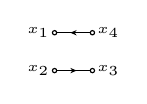
\begin{tikzpicture}[x=0.340cm, y=0.340cm, line width=0.420pt, baseline={([yshift=-0.6ex]0,0)}]
  \draw (0.707,0.707) -- (-0.707,0.707);
  \fill (-0.119,0.707) -- (0.119,0.605) -- (0.042,0.707) -- (0.119,0.809) -- cycle;
  \draw (-0.707,-0.707) -- (0.707,-0.707);
  \fill (0.119,-0.707) -- (-0.119,-0.605) -- (-0.042,-0.707) -- (-0.119,-0.809) -- cycle;
  \draw[fill=white] (-0.707,0.707) circle (0.080);
  \draw[fill=white] (-0.707,-0.707) circle (0.080);
  \draw[fill=white] (0.707,-0.707) circle (0.080);
  \draw[fill=white] (0.707,0.707) circle (0.080);
  \node[font=\tiny, inner sep=0pt, anchor=0] at (-0.877,0.707) {$x_{1}$};
  \node[font=\tiny, inner sep=0pt, anchor=0] at (-0.877,-0.707) {$x_{2}$};
  \node[font=\tiny, inner sep=0pt, anchor=180] at (0.877,-0.707) {$x_{3}$};
  \node[font=\tiny, inner sep=0pt, anchor=180] at (0.877,0.707) {$x_{4}$};
\end{tikzpicture}}
\diagramgap
\mbox{$\displaystyle -\,$\,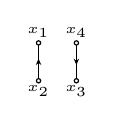
\begin{tikzpicture}[x=0.340cm, y=0.340cm, line width=0.420pt, baseline={([yshift=-0.6ex]0,0)}]
  \draw (-0.707,-0.707) -- (-0.707,0.707);
  \fill (-0.707,0.119) -- (-0.809,-0.119) -- (-0.707,-0.042) -- (-0.605,-0.119) -- cycle;
  \draw (0.707,0.707) -- (0.707,-0.707);
  \fill (0.707,-0.119) -- (0.809,0.119) -- (0.707,0.042) -- (0.605,0.119) -- cycle;
  \draw[fill=white] (-0.707,0.707) circle (0.080);
  \draw[fill=white] (-0.707,-0.707) circle (0.080);
  \draw[fill=white] (0.707,-0.707) circle (0.080);
  \draw[fill=white] (0.707,0.707) circle (0.080);
  \node[font=\tiny, inner sep=0pt, anchor=270] at (-0.707,0.877) {$x_{1}$};
  \node[font=\tiny, inner sep=0pt, anchor=90] at (-0.707,-0.877) {$x_{2}$};
  \node[font=\tiny, inner sep=0pt, anchor=90] at (0.707,-0.877) {$x_{3}$};
  \node[font=\tiny, inner sep=0pt, anchor=270] at (0.707,0.877) {$x_{4}$};
\end{tikzpicture}}
